\subsection{Peak Ratio}\label{subsec:peakratio}

The Sandvine Reports show that although the mean traffic demand has remained
stable for the past few years, demand during prime-time hours has increased
drastically~\cite{sandvine20141h}. These reports present a good view 
into aggregate usage patterns over a month, however they neglect to analyze usage
characteristics per subscriber.
We measure the disparity between the daily 95 percentile of the peak and 
mean usage of each household, and call this the \emph{Peak-Ratio}.

\begin{figure}[t]
\begin{minipage}{1\linewidth}
\centering
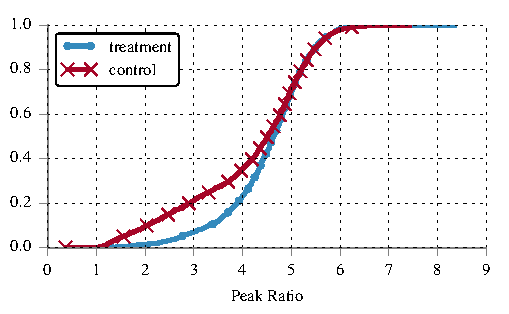
\includegraphics[width=1\linewidth]{figures/peakratio_cdf_mean-devices.pdf}
\caption{Distribution of the average peak ratio per subscriber in the treatment and 
control groups.}
\label{fig:CDF-peak-ratio-mean}
\end{minipage}
\end{figure}

Figure ~\ref{fig:CDF-peak-ratio-mean} plots the peak-ratio for each 
subscriber in the \treatment{} and \control{} sets. The median peak
ratio for subscribers from the higher and lower tier is 4.64 and 4.51
respectively. Subscribers with a higher daily peak ratio have similar
peak ratios in both the sets. However, 40 percent of the subscribers
in the \control{} group have a lower peak ratio than the lowest 40\% of
the \treatment{} group. Further analysis showed that weekdays have 
the most disparity between peak ratios, whereas on weekends peak ratios
for both \control{} and \treatment{} group are similar.